% Poster A2 (420x594 mm), tiếng Việt — dịch bằng tectonic:  make poster-pdf
% Mọi số liệu lấy từ docs/competition/competition-claims.md (đã kiểm). Công suất: đã đo 29/10 (docs/energy-2026-10-29).
\documentclass[24pt]{extarticle}
\usepackage{fontspec}
\setmainfont{Liberation Sans}
\usepackage{polyglossia}
\setmainlanguage{vietnamese}
\usepackage[paperwidth=420mm,paperheight=594mm,margin=8mm]{geometry}
\usepackage{xcolor}
\usepackage{tikz}
\usetikzlibrary{arrows.meta,positioning}
\usepackage{pgfplots}
\pgfplotsset{compat=1.17}
\pgfplotsset{
  ch/.style={ybar,width=\linewidth,height=36mm,bar width=10mm,ymin=0,enlarge x limits=0.2,
    /pgf/number format/use comma,
    x tick label style={font=\fontsize{13}{16}\selectfont},yticklabel style={font=\fontsize{14}{17}\selectfont},
    ylabel style={font=\fontsize{16}{19}\selectfont},xlabel style={font=\fontsize{16}{19}\selectfont},
    title style={font=\fontsize{19}{23}\selectfont\bfseries},
    nodes near coords style={font=\fontsize{16}{19}\selectfont\bfseries,text=black},
    ytick=\empty,yticklabels={},axis line style={gray!70}}}
\usepackage[most]{tcolorbox}
\usepackage{enumitem}
\usepackage{booktabs,array}
\usepackage{graphicx}
\pagestyle{empty}
\setlength{\parindent}{0pt}
\setlength{\parskip}{2pt}
\raggedright
\setlist{itemsep=3pt,topsep=2pt,leftmargin=1.1em}

\definecolor{navy}{HTML}{16324F}
\definecolor{teal}{HTML}{0E7C86}
\definecolor{okg}{HTML}{2E9E4F}
\definecolor{wrn}{HTML}{E0A100}
\definecolor{crit}{HTML}{C62828}
\definecolor{mute}{HTML}{6B7280}
\definecolor{paper}{HTML}{F4F6F8}

\tcbset{
  sec/.style={enhanced,colback=white,colframe=navy,boxrule=1.4pt,arc=3mm,
    fonttitle=\bfseries\fontsize{25}{29}\selectfont,coltitle=white,colbacktitle=navy,
    attach boxed title to top left={xshift=6mm,yshift=-5mm},
    boxed title style={arc=2.5mm,boxrule=0pt,left=5mm,right=5mm,top=1.5mm,bottom=1.5mm},
    top=8mm,left=6mm,right=6mm,bottom=4mm,before skip=9pt,after skip=0pt,
    fontupper=\fontsize{18}{21.5}\selectfont}
}
\newcommand{\num}[1]{{\bfseries\color{teal}#1}}
\newcommand{\kpi}[2]{\begin{minipage}[t]{0.157\linewidth}\begin{tcolorbox}[enhanced,colback=teal!9,colframe=teal!9,boxrule=0pt,arc=2.5mm,left=1mm,right=1mm,top=1.5mm,bottom=1.5mm,halign=center,before skip=0pt,after skip=0pt]
{\fontsize{28}{31}\selectfont\bfseries\color{teal}#1}\\[-1mm]{\fontsize{15}{17}\selectfont\color{navy}#2}\end{tcolorbox}\end{minipage}}
\newcommand{\pcap}[1]{{\fontsize{16}{19}\selectfont\color{mute}#1}}

\begin{document}
\pagecolor{paper}
\begin{tcolorbox}[enhanced,colback=navy,colframe=navy,arc=5mm,left=12mm,right=12mm,top=3mm,bottom=3mm,before skip=0pt,after skip=0pt]
{\color{white}\raggedright
{\fontsize{20}{24}\selectfont\color{white!78!navy} EDGE AI DESIGN CHALLENGE 2026 \enspace|\enspace Khoa Điện -- Điện tử, ĐH Công nghệ Kỹ thuật TP.HCM}\\[0.5mm]
{\fontsize{34}{39}\selectfont\bfseries EDGE AI SMART LABORATORY SAFETY MONITORING SYSTEM}\\[0.5mm]
{\fontsize{20}{24}\selectfont Hệ thống AI biên cảnh báo người \emph{không mặc áo blouse} trong vùng nguy hiểm, xử lý tại chỗ trên NPU của Orange Pi 5, không cần Internet (mạng chỉ dùng cho tin Zalo)}\\[1mm]
{\fontsize{20}{24}\selectfont\textbf{Lê Tự Thiện An (nhóm trưởng)} \enspace|\enspace Trịnh Anh Văn \enspace|\enspace Võ Nhật Nam \enspace|\enspace Phạm Trọng Thành}}
\end{tcolorbox}

% ---------------------------------------------------------------- hàng 1
\begin{minipage}[t]{0.485\textwidth}
\vspace{0pt}
\begin{tcolorbox}[sec,title={1. Bài toán và ý tưởng}]
Việc nhắc nhở bằng người khó duy trì liên tục, còn gửi video lên đám mây thì tốn băng thông và lộ hình ảnh người trong phòng. Nhóm xây dựng một thiết bị dùng Orange Pi 5 và camera USB để nhận biết người có mặc \emph{áo blouse} hay không, và cảnh báo khi người \emph{không mặc áo} bước vào \emph{vùng nguy hiểm} do người dùng tự vẽ.
\end{tcolorbox}

\begin{tcolorbox}[sec,title={2. Đóng góp kỹ thuật chính}]
\begin{enumerate}[leftmargin=1.4em,itemsep=2pt]
  \item \textbf{Kiểm tra tương đương NPU--CPU.} Đầu ra trên NPU được so với CPU trước khi dùng; cách này phát hiện \num{4 lỗi chuyển đổi} mà tốc độ không phản ánh.
  \item \textbf{Lượng tử hóa INT8 với đầu ra tách.} Tách khung và điểm lớp thành 6 tensor: mAP50-95 chỉ giảm khoảng \num{1 điểm} thay vì \num{17--20 điểm}.
  \item \textbf{Chế độ thích nghi.} Mô hình phụ chỉ chạy khi cần, trên nhân NPU riêng. So với chế độ song song: NPU \num{32} so với 74 ms/khung, nhiệt độ thấp hơn \num{12,8\,$^\circ$C}, công suất \num{1,98 W} so với \num{3,34 W}.
  \item \textbf{Chỉ kết luận khi thấy rõ trang phục.} Người chỉ lộ mặt hoặc bị che được đánh dấu ``chưa thấy rõ áo''; trên video lab đông người, số cảnh báo giảm từ \num{31 xuống 6}, cả 6 đều đúng.
  \item \textbf{Dữ liệu ít nhãn.} Chọn đúng ảnh khó và thêm mẫu âm tính từ COCO: lỗi nhận nhầm áo thun trắng là áo blouse giảm từ \num{20/20 xuống 0--4/20}.
\end{enumerate}
\end{tcolorbox}
\end{minipage}\hfill
\begin{minipage}[t]{0.485\textwidth}
\vspace{0pt}
\begin{tcolorbox}[sec,title={3. Kiến trúc và luồng xử lý}]
\centering
\begin{minipage}[t]{0.243\linewidth}\centering\vspace{0pt}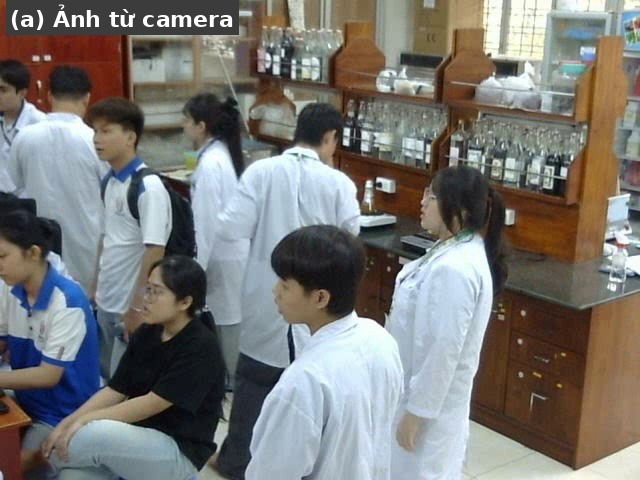
\includegraphics[width=\linewidth]{img/pipe_a.jpg}\\[0.5mm]{\fontsize{15}{17}\selectfont\color{navy}\textbf{1.} Camera USB 30 FPS}\end{minipage}\hfill
\begin{minipage}[t]{0.243\linewidth}\centering\vspace{0pt}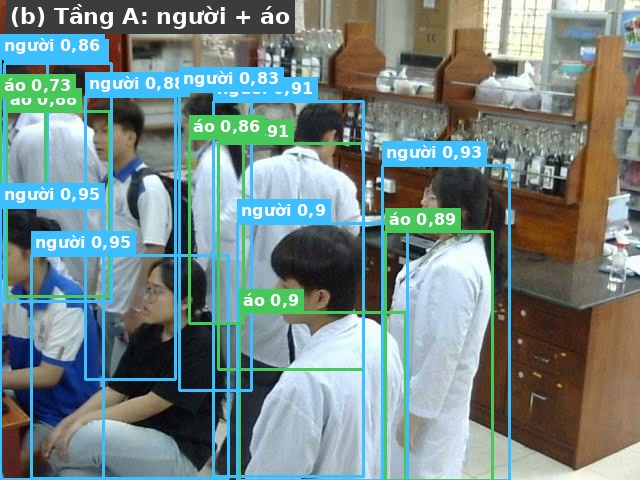
\includegraphics[width=\linewidth]{img/pipe_b.jpg}\\[0.5mm]{\fontsize{15}{17}\selectfont\color{navy}\textbf{2.} Tầng A: YOLO26n INT8 trên NPU}\end{minipage}\hfill
\begin{minipage}[t]{0.243\linewidth}\centering\vspace{0pt}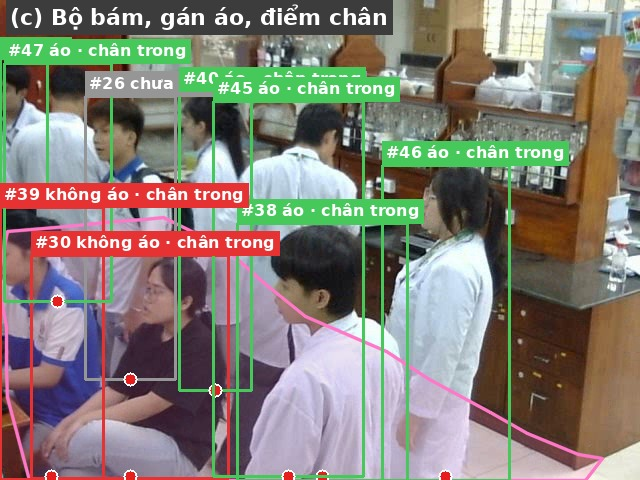
\includegraphics[width=\linewidth]{img/pipe_c.jpg}\\[0.5mm]{\fontsize{15}{17}\selectfont\color{navy}\textbf{3.} Theo vết, gán áo, điểm chân}\end{minipage}\hfill
\begin{minipage}[t]{0.243\linewidth}\centering\vspace{0pt}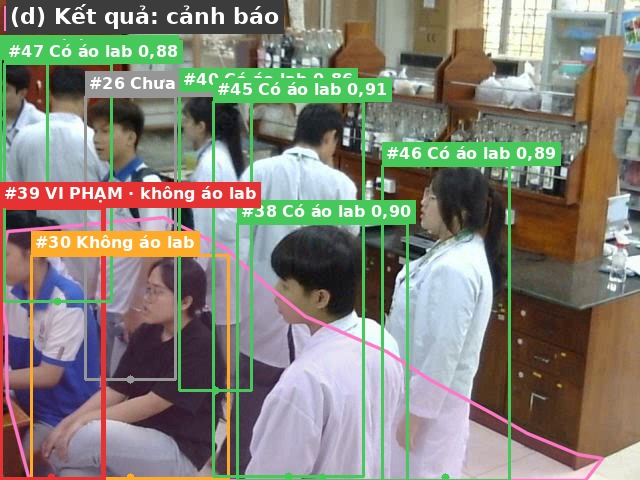
\includegraphics[width=\linewidth]{img/pipe_d.jpg}\\[0.5mm]{\fontsize{15}{17}\selectfont\color{navy}\textbf{4.} Xác nhận 3 s $\to$ web, LED, OLED, Zalo}\end{minipage}\\[1mm]
\pcap{Một khung hình thật qua từng bước xử lý. Báo động khi người ở trong vùng, không mặc áo và nhìn thấy rõ trang phục.}
\end{tcolorbox}

\begin{tcolorbox}[sec,title={4. Ưu điểm của thiết kế}]
\begin{itemize}
  \item \textbf{Riêng tư, không phụ thuộc mạng:} xử lý trên NPU của bo mạch, không gửi hình ra ngoài; chỉ tin Zalo cần Internet.
  \item \textbf{Tin cậy khi không chắc chắn:} mất hình không báo AN TOÀN; chưa thấy rõ áo thì không kết luận vi phạm.
  \item \textbf{Nhanh và tiết kiệm điện:} 29 khung/giây, độ trễ p99 41,4 ms, chỉ 2,2 W.
  \item \textbf{Dễ triển khai:} vẽ vùng nguy hiểm ngay trên trang web; tự khởi động khi cấp điện.
\end{itemize}
\end{tcolorbox}
\end{minipage}

% ---------------------------------------------------------------- hàng 2: kết quả
\begin{tcolorbox}[sec,title={5. Kết quả đo trên thiết bị thật}]
% ---- hàng đồ thị A
\begin{minipage}[t]{0.325\linewidth}
\vspace{0pt}\centering
\begin{tikzpicture}
\begin{axis}[ch,ymax=42,symbolic x coords={CPU,NPU,Có web,Camera},xtick=data,title={Tốc độ xử lý},ylabel={khung/giây},nodes near coords]
\addplot[fill=teal!80,draw=navy] coordinates {(CPU,10.5) (NPU,29.0) (Có web,25.9) (Camera,30)};
\end{axis}
\end{tikzpicture}\\
\pcap{Video phát lại: p99 \num{41,4 ms}, \num{25,9 FPS} khi bật web. CPU (FP32) chỉ 10,5 FPS, nóng 86,8\,$^\circ$C.}
\end{minipage}\hfill
\begin{minipage}[t]{0.325\linewidth}
\vspace{0pt}\centering
\begin{tikzpicture}
\begin{axis}[ch,ymax=0.95,bar width=11mm,symbolic x coords={FP32,INT8 thường,INT8 tách},xtick={FP32,INT8 thường,INT8 tách},title={Độ chính xác sau INT8},ylabel={mAP50-95},enlarge x limits=0.3,bar shift=0pt,nodes near coords]
\addplot[fill=navy!70,draw=navy] coordinates {(FP32,0.661) (INT8 thường,0.48)};
\addplot[fill=okg,draw=navy] coordinates {(INT8 tách,0.657)};
\end{axis}
\end{tikzpicture}\\
\pcap{Góc camera 1, tập kiểm tra độc lập. INT8 mặc định mất 18 điểm, đầu ra tách chỉ mất 0,4 điểm.}
\end{minipage}\hfill
\begin{minipage}[t]{0.325\linewidth}
\vspace{0pt}\centering
\begin{tikzpicture}
\begin{axis}[ch,ymax=5.2,bar width=9mm,bar shift=0pt,symbolic x coords={Nghỉ,Sản phẩm,Thích nghi,Song song},xtick={Nghỉ,Sản phẩm,Thích nghi,Song song},x tick label style={font=\fontsize{12}{15}\selectfont},title={Công suất điện},ylabel={watt (W)},enlarge x limits=0.15,
  nodes near coords={\pgfmathprintnumber[use comma,fixed,fixed zerofill,precision=2]{\pgfplotspointmeta}}]
\addplot[fill=mute!70,draw=navy] coordinates {(Nghỉ,0.86)};
\addplot[fill=teal!80,draw=navy] coordinates {(Sản phẩm,2.20)};
\addplot[fill=okg,draw=navy] coordinates {(Thích nghi,1.98)};
\addplot[fill=crit!80,draw=navy] coordinates {(Song song,3.34)};
\end{axis}
\end{tikzpicture}\\
\pcap{Đồng hồ USB-C, video phát lại, sai số $\pm$10\%. Thích nghi tiết kiệm \num{1,36 W} (41\%) so với song song.}
\end{minipage}\\[4mm]
% ---- hàng đồ thị B
\begin{minipage}[t]{0.325\linewidth}
\vspace{0pt}\centering
\begin{minipage}[t]{0.49\linewidth}\centering
\begin{tikzpicture}
\begin{axis}[ch,height=36mm,ymax=100,bar width=9mm,bar shift=0pt,symbolic x coords={Thích nghi,Song song},xtick={Thích nghi,Song song},x tick label style={font=\fontsize{11}{13}\selectfont},title={\fontsize{16}{19}\selectfont NPU (ms/khung)},enlarge x limits=0.5,nodes near coords]
\addplot[fill=okg,draw=navy] coordinates {(Thích nghi,32)};
\addplot[fill=crit!80,draw=navy] coordinates {(Song song,74)};
\end{axis}
\end{tikzpicture}
\end{minipage}\hfill
\begin{minipage}[t]{0.49\linewidth}\centering
\begin{tikzpicture}
\begin{axis}[ch,height=36mm,ymin=30,ymax=68,bar width=9mm,bar shift=0pt,symbolic x coords={Thích nghi,Song song},xtick={Thích nghi,Song song},x tick label style={font=\fontsize{11}{13}\selectfont},title={\fontsize{16}{19}\selectfont Nhiệt SoC ($^\circ$C)},enlarge x limits=0.5,nodes near coords]
\addplot[fill=okg,draw=navy] coordinates {(Thích nghi,41.5)};
\addplot[fill=crit!80,draw=navy] coordinates {(Song song,54.3)};
\end{axis}
\end{tikzpicture}
\end{minipage}\\
\pcap{Thích nghi so với song song, 3 lượt $\times$ 15 phút: ít tính toán hơn 2,3 lần, mát hơn \num{12,8\,$^\circ$C}.}
\end{minipage}\hfill
\begin{minipage}[t]{0.325\linewidth}
\vspace{0pt}\centering
\begin{tikzpicture}
\begin{axis}[ch,ymax=118,bar width=7mm,bar shift=0pt,nodes near coords style={font=\fontsize{14}{16}\selectfont\bfseries,text=black},symbolic x coords={Góc 1,Góc 2},xtick={Góc 1,Góc 2},title={Luật vùng (ngưỡng áo 0,6)},ylabel={\%},enlarge x limits=0.45,
  nodes near coords={\pgfmathprintnumber[fixed,precision=0]{\pgfplotspointmeta}},ytick=\empty]
\addplot[fill=okg,draw=navy,bar shift=-4mm] coordinates {(Góc 1,81) (Góc 2,88)};
\addplot[fill=crit!80,draw=navy,bar shift=4mm] coordinates {(Góc 1,8) (Góc 2,10)};
\end{axis}
\end{tikzpicture}\\
\pcap{\textcolor{okg}{\textbf{Xanh}}: phát hiện người không áo. \textcolor{crit}{\textbf{Đỏ}}: báo nhầm người có áo. Theo từng người, INT8 trên NPU, TB 3 lần. Còn bỏ sót.}
\end{minipage}\hfill
\begin{minipage}[t]{0.325\linewidth}
\vspace{0pt}\centering
\begin{tikzpicture}
\begin{axis}[width=\linewidth,height=36mm,xmin=0,xmax=24,ymin=0,ymax=300,/pgf/number format/use comma,
  title={RAM trong 24 giờ},title style={font=\fontsize{19}{23}\selectfont\bfseries},
  xlabel={giờ chạy liên tục},ylabel={RSS (MB)},xlabel style={font=\fontsize{16}{19}\selectfont},ylabel style={font=\fontsize{16}{19}\selectfont},
  xticklabel style={font=\fontsize{14}{17}\selectfont},yticklabel style={font=\fontsize{14}{17}\selectfont},xtick={0,6,12,18,24},ytick={0,100,200,300},ymajorgrids,grid style={gray!25}]
\addplot[teal,line width=2pt,no marks] table[x=h,y=rss] {ram24h.dat};
\end{axis}
\end{tikzpicture}\\
\pcap{Chạy liên tục 24 giờ: RAM ổn định 210--220 MB, cao nhất 269 MB, không lỗi.}
\end{minipage}
\end{tcolorbox}

% ---------------------------------------------------------------- hàng 3
\begin{minipage}[t]{0.585\textwidth}
\vspace{0pt}
\begin{tcolorbox}[sec,title={6. Sản phẩm demo và chức năng}]
\begin{minipage}[t]{0.25\linewidth}
\vspace{0pt}
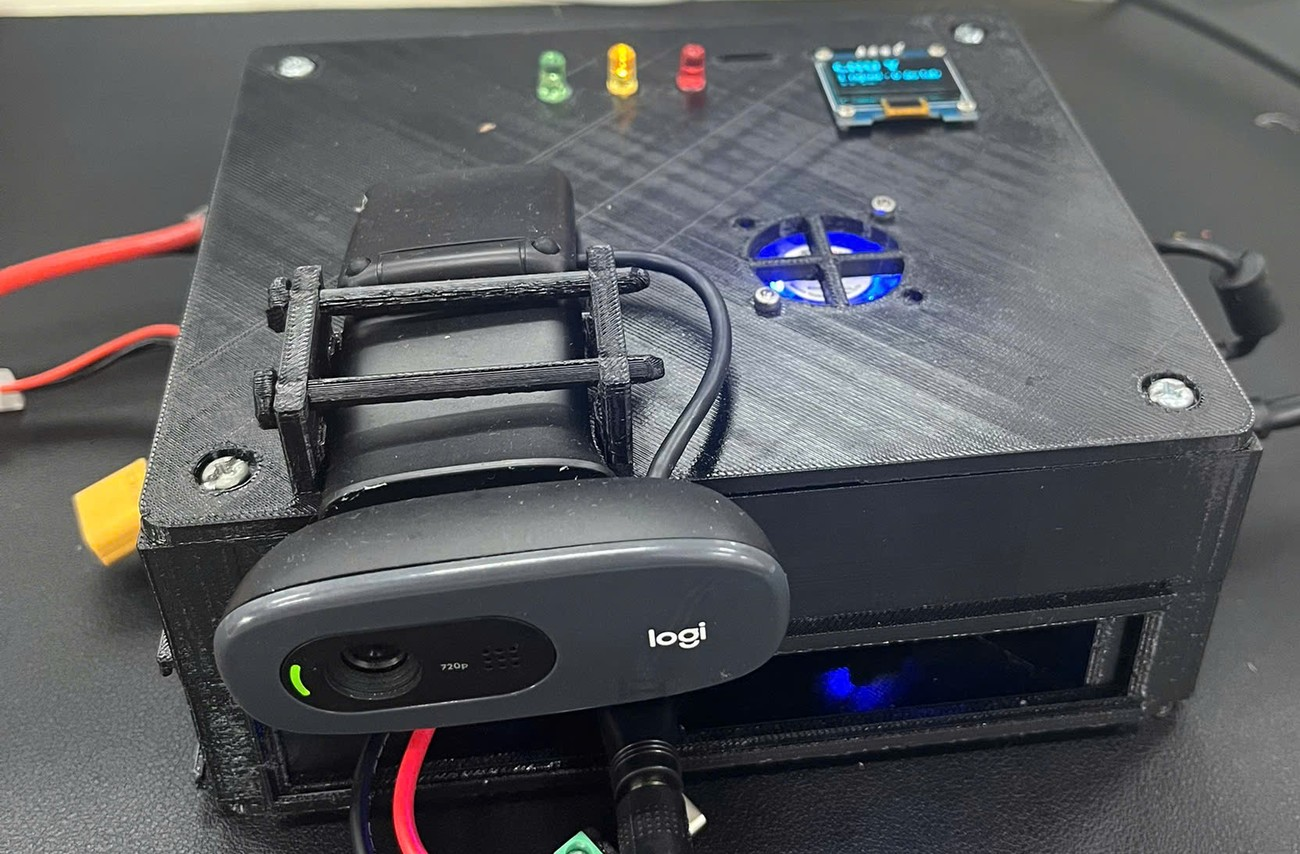
\includegraphics[width=\linewidth]{img/hardware_full.jpg}\\[0.5mm]
\pcap{Thiết bị: vỏ in 3D, camera, 3 LED, OLED.}
\end{minipage}\hfill
\begin{minipage}[t]{0.40\linewidth}
\vspace{0pt}
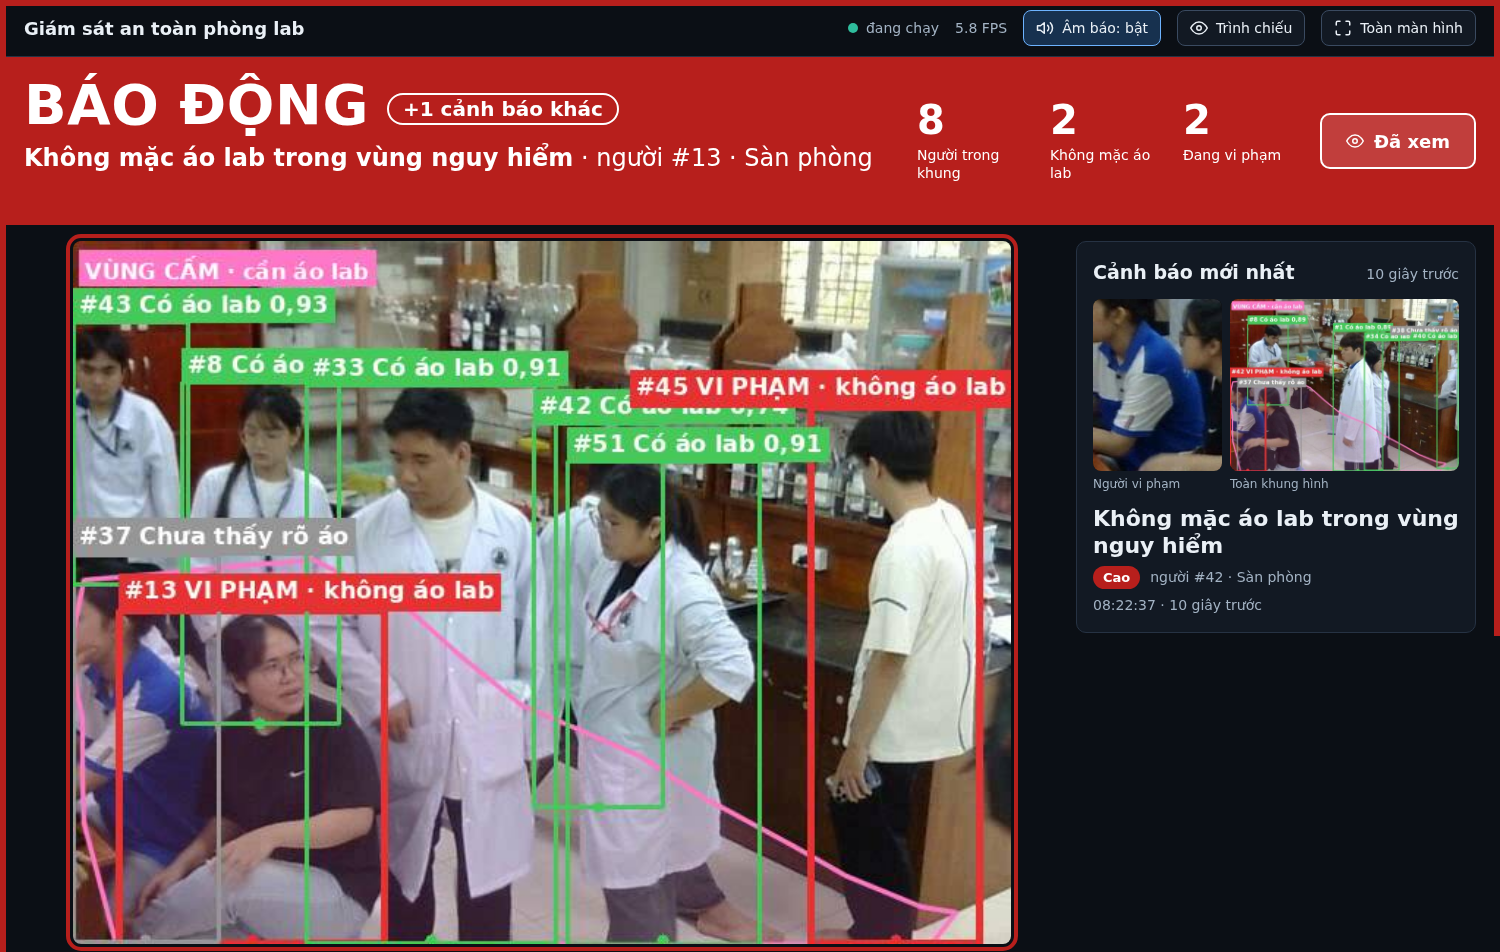
\includegraphics[width=\linewidth]{img/dashboard.png}\\[0.5mm]
\pcap{Trang web khi báo động.}
\end{minipage}\hfill
\begin{minipage}[t]{0.21\linewidth}
\vspace{0pt}
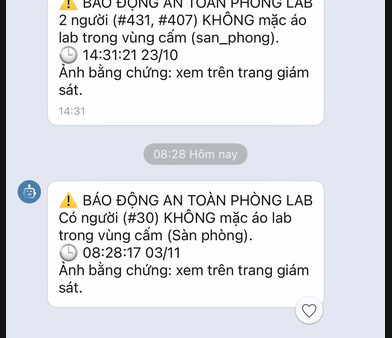
\includegraphics[width=\linewidth]{img/zalo_crop.png}\\[0.5mm]
\pcap{Tin nhắn Zalo.}
\end{minipage}\hfill\\[2mm]
\begin{minipage}[t]{\linewidth}
{\fontsize{18}{22}\selectfont
\textbf{4 trạng thái} (web, đèn, OLED):\\[0.5mm]
\colorbox{okg}{\textcolor{white}{\strut\,AN TOÀN\,}} \colorbox{wrn}{\strut\,CHÚ Ý\,} \colorbox{crit}{\textcolor{white}{\strut\,BÁO ĐỘNG\,}} \colorbox{mute}{\textcolor{white}{\strut\,MẤT TÍN HIỆU\,}}\\[0.5mm]
Mất hình không bao giờ báo AN TOÀN.\\[1mm]
\textbf{Chức năng:} phát hiện người và áo blouse \textbullet\ vẽ vùng ngay trên web \textbullet\ cảnh báo qua web, đèn, OLED, Zalo \textbullet\ lưu ảnh bằng chứng \textbullet\ tự khởi động khi cấp điện.}
\end{minipage}
\end{tcolorbox}
\end{minipage}\hfill
\begin{minipage}[t]{0.385\textwidth}
\vspace{0pt}
\begin{tcolorbox}[sec,colframe=wrn!80!black,colbacktitle=wrn!80!black,coltitle=black,title={7. Giới hạn và hướng phát triển}]
\begin{itemize}
  \item \textbf{Góc camera ảnh hưởng lớn:} ở góc quá khác dữ liệu huấn luyện, mô hình không nhận ra áo (0/122 khung); đưa camera về góc cũ thì nhận được 98\% (thử 25 giây, chưa phải độ chính xác).
  \item Hai người đứng sát nhau có thể bị gán nhầm áo trong tối đa 2 giây.
  \item Công suất đo trên video phát lại, mỗi chế độ một lần, chưa tính camera.
  \item Té ngã, lửa và khói đã có mã nguồn nhưng \textbf{đang tắt}, chưa đánh giá thực tế.
  \item \textbf{Hướng phát triển:} thu thêm dữ liệu tại vị trí lắp đặt, đo công suất với camera thật, thử cắt tỉa và chưng cất tri thức.
\end{itemize}
\end{tcolorbox}
\end{minipage}

\end{document}
